%
	\chapter*{Motivation}\addchaptertocentry{Motivation}
%
%       WOMIT SICH DIE ARBEIT BESCHÄFTIGT UND WARUM DAS INTERESSANT IST
%       FORMULIERUNG DER HAUPTFRAGESTELLUNGEN (HÖCHSTENS 3), DIE DANN BEARBEITET WERDEN 
%       (IN DER SUMMARY DANN DIESE BEANTWORTEN)
%       DARAUS ABLEITUNG DER GLIEDERUNG DER ARBEIT: GRUNDLAGEN, METHODEN, 1D FÜR REFERENZ
%       DARAUS 2D ABSOLUT NÖTIG WEGEN ASYMMETRIE-EFFEKTEN UND SELF-BIAS,
%       ZUSAMMENFASSUNG UND OUTLINE
%
        Reactive plasmas are a common tool in many industrial and scientific applications, such as semiconductor and computer chip production. Of high importance for the surface treatment are etching and sputtering processes~\cite{Cvelbar05,Zeuner98}. Especially in electronegative discharges sputter and deposition rates are increased. Therefore a deep interest in the energy distribution function (EDF) of the charged plasma species exists. Capacitively coupled discharges with radio-frequency modulated voltages (ccrf) have high-energy ions impinging on the electrodes. Their advantage is that there is no net current, which preserves the structure of the target --- for example, the target would be one of the electrodes, or placed there-on.\\
        Laboratory experiments with ccrf oxygen discharges at low pressures and temperatures have shown a high-energy peak in the EDF of negative ions impinging on the anode. The position of this peak depends on the electrode material~\cite{Scheuer15}. Experimentally measured anion EDF is shown in~\autoref{fig:anionedf_scheuer}. A possible explanation is proposed by Stoffels and Kawano et al.~\cite{Stoffels01,Kawano83}: negative ions are produced by ionisation close to or at the surface of the electrode. The drawback of this theory is the lack of experimental or theoretical ionisation probabilities for anions at metal surfaces. Until now an explanation for this characteristic of the incident negative ion EDF at the anode is missing.
%
        \begin{figure}[!h]
            \centering
            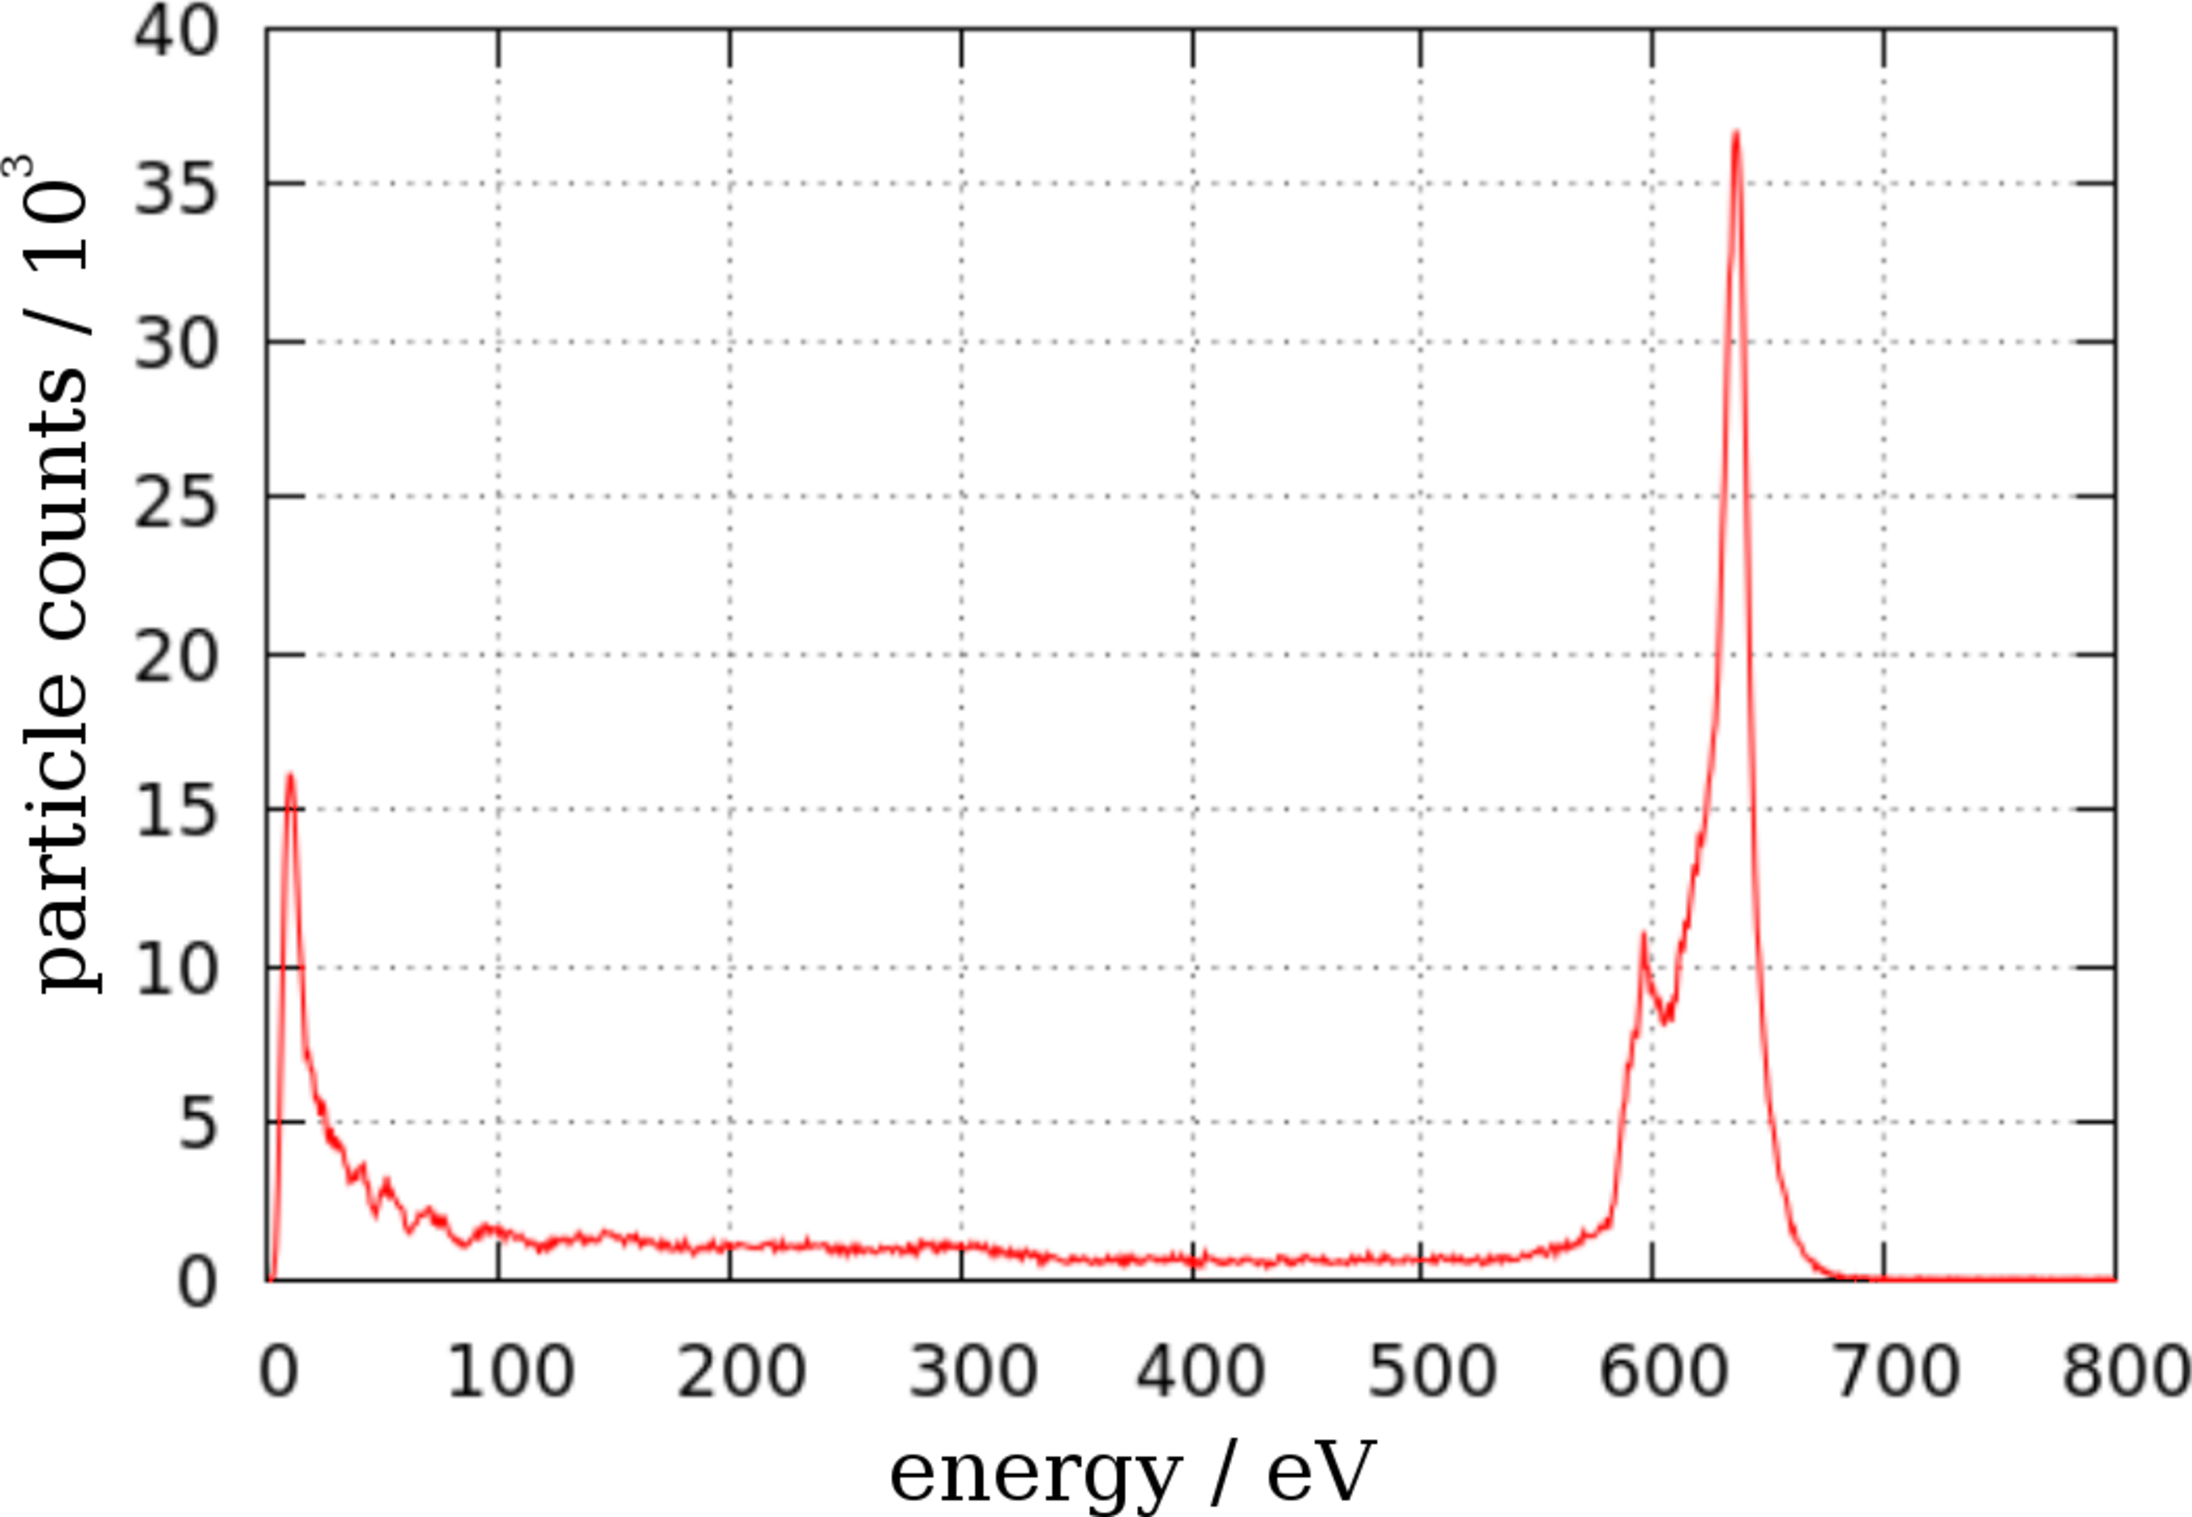
\includegraphics[width=0.6\textwidth]{figures/scheuer_anionedf.pdf}
            \caption{Experimentally measured anion energy distribution function impinging on the grounded electrode. Magnesium oxyde was used as the cathode material, which was powered with $\SI{50}{\watt}$~\cite{Scheuer15}.}
            \label{fig:anionedf_scheuer}
        \end{figure}
%        
        In my thesis I will try to reproduce the experimental investigations and verify or falsify the theoretical model. Therefore a Particle-in-Cell (PIC) computer simulation with a Monte-Carlo-Collisions (MCC) algorithm is used to model the asymmetric ccrf discharge with low-temperature oxygen plasmas. Hence an additional surface ionisation channel for negative ions is introduced to the simulation.\\
        Numerical investigations of electronegative plasmas have been done, e.g.\@ by~\cite{Matyash07oxIII,Bronold07b,Matthias15} using an one-dimensional PIC model. It has proven to be a great tool for simple and fundamental studies of reactive radio frequency plasmas. Their results have been widely approved. Though this is a good approach for the investigation of axial distribution functions of plasma species, the 1D simulations lacks effects of asymmetry and plasma-wall interaction. Therefore I will compare the one- and two-dimensional simulation results, which allows an improved understanding of the processes determining the dynamics of negative ions. In the 2D model, additional characteristics, such as voltage offset \emph{self bias} in ccrf discharges and asymmetry effects are implemented.\\
        \newline
        In this thesis I will first introduce the underlying physics of radio frequency plasmas and the unique features of asymmetric, capacitively coupled discharges. Of special interest is the plasma-wall interaction. Here, corresponding particle fluxes, potential, densities and secondary emission processes will be discussed. Subsequently the PIC simulation method is introduced. I will highlight the limits and advantages of both 1D and 2D algorithms, as well as the transition between them. Conclusively, an excerpt from the full oxygen reaction set is compiled with respect to their importance to the investigated plasma discharges.\\
        In the first part of my analysis I will simulate the axial centre of the discharge without asymmetry effects using the one-dimensional model. These results are compared the 2D expansion of the simulation. Thereby I will try to show the validity of the two-dimensional PIC method. Afterwards this model is used to simulate the plasma discharge from~\cite{Scheuer15}. The investigation of surface and asymmetry effects and their impact on the discharge is the goal of this work.